% begin cgal manual page

\begin{ccRefClass}{PM_explorer}\ccCreationVariable{E}

\ccSection{Plane map exploration}

\ccDefinition

An instance \ccc{E} of the data type \ccc{PM_explorer} is a decorator
to explore the structure of the plane map underlying the Nef
polyhedron. It inherits all topological adjacency exploration
operations from \ccc{PM_const_decorator}. \ccc{PM_explorer}
additionally allows to explore the geometric embedding.

The position of each vertex is given by a so-called extended point, which is
either a standard affine point or the tip of a ray touching an
infinimaximal quadratic frame centered at the origin. A vertex \ccc{v} is
called a \emph{standard} vertex if its embedding is a \emph{standard}
point and \emph{non-standard} if its embedding is a
\emph{non-standard} point. By the embedding of their source and target
vertices edges correspond to either affine segments, rays or lines
or are part of the bounding frame.
%\providecommand{\displayeps}[3]{}
%\providecommand{\manfigref}[1]{}
%\manfigref{See figure \figref{extsegs}.}

\begin{figure}[htbp]
\begin{ccTexOnly}
\begin{center}
\scalebox{0.5}{\includegraphics{Nef_2_ref/extsegs.eps}}
\end{center}
\end{ccTexOnly}
\caption{Extended geometry: standard vertices are marked
by S, non-standard vertices are marked by N. \textbf{A}: The possible
embeddings of edges: an affine segment s1, an affine ray s2, an affine
line s3. \textbf{B}: A plane map embedded by extended geometry: note
that the frame is arbitrary large, the 6 vertices on the frame are at
infinity, the two faces represent a geometrically unbounded area,
however they are topologically closed by the frame edges. No standard
point can be placed outside the frame.}
\label{extsegs}    
\begin{ccHtmlOnly}
<CENTER>
<IMG BORDER=0 SRC="./extsegs.gif" ALIGN=center
ALT="Extended geometry">
</CENTER>
\end{ccHtmlOnly}
\end{figure}

\ccInheritsFrom{PM\_const\_decorator}

\ccSetOneOfTwoColumns{4cm}

\ccTypes

\ccNestedType{Point}{the point type of finite vertices. 
}

\ccNestedType{Ray}{the ray type of vertices on the frame. 
}

Iterators, handles, and circulators are inherited from 
\ccc{PM_const_decorator}. 



\ccSetOneOfTwoColumns{3cm}

\ccCreation

\ccc{PM_explorer} is copy constructable and assignable. An object
can be obtained via the \ccc{Nef_polyhedron_2::explorer()} method of
\ccc{Nef_polyhedron_2}. 



\ccSetOneOfTwoColumns{2cm}

\ccOperations

\ccMethod{bool is_standard(Vertex_const_handle v) ;}{returns true iff \ccc{v}'s position is a standard point. 
}

\ccMethod{Point point(Vertex_const_handle v) ;}{returns the standard point that is the embedding of \ccc{v}.
\ccPrecond \ccc{E.is_standard(v)}. 
}

\ccMethod{Ray ray(Vertex_const_handle v) ;}{returns the ray defining the non-standard point on the frame. 
\ccPrecond \ccc{!E.is_standard(v)}. 
}

\ccMethod{bool is_frame_edge(Halfedge_const_handle e) ;}{returns true iff \ccc{e} is part of the infinimaximal frame. 
}

\end{ccRefClass}


